\documentclass[10pt]{article}
%\usepackage[left=2.3cm,right=2.3cm,top=2.5cm,bottom=3cm,a4paper]{geometry}
\usepackage{fullpage}
\usepackage{setspace}
\setstretch{1.3}
\usepackage{amsmath,amssymb,amsthm,physics,units}
\usepackage[shortlabels]{enumitem}
\setlength\parindent{0pt}
\usepackage{graphicx,float,subcaption,multirow}
\DeclareGraphicsExtensions{.pdf,.png,.jpg,.jpeg}
\usepackage{float}
\usepackage{algorithm,algpseudocode}
\usepackage[shortlabels]{enumitem}
\usepackage{hyperref}
\hypersetup{
    colorlinks=true,
    linkcolor=black,
    filecolor=black,      
    urlcolor=black,
    pdftitle={Overleaf Example},
    pdfpagemode=FullScreen,
}

\begin{document}
\begin{center}
    {\LARGE Engineering Mathematics 1 Problem Set 2} \\
\end{center}
\begin{flushright}
    Department of Computer Science and Engineering \\
    2021-16988 Jaewan Park
\end{flushright}

\section*{Problem 1}
\begin{enumerate}[leftmargin=*, label={(\alph*)}]
    \item The characteristic polynomial of $\mathbf{A}$ is 
    \begin{align*}
        D(\lambda) &= \begin{vmatrix}
            a_{11} - \lambda & a_{12} & a_{13} & \cdots & a_{1n} \\
            a_{21} & a_{22} - \lambda & a_{23} & \cdots & a_{2n} \\ 
            a_{31} & a_{32} & a_{33} - \lambda & \cdots & a_{3n} \\ 
            \vdots & \vdots & \vdots & \ddots & \vdots \\
            a_{n1} & a_{n2} & a_{n3} & \cdots & a_{nn} - \lambda
        \end{vmatrix} \\
        &= \qty(a_{11} - \lambda)\begin{vmatrix}
            a_{22} - \lambda & a_{23} & \cdots & a_{2n} \\ 
            a_{32} & a_{33} - \lambda & \cdots & a_{3n} \\ 
            \vdots & \vdots & \ddots & \vdots \\
            a_{n2} & a_{n3} & \cdots & a_{nn} - \lambda
        \end{vmatrix} - a_{21}\begin{vmatrix}
            a_{12} & a_{13} & \cdots & a_{1n} \\
            a_{32} & a_{33} - \lambda & \cdots & a_{3n} \\ 
            \vdots & \vdots & \ddots & \vdots \\
            a_{n2} & a_{n3} & \cdots & a_{nn} - \lambda
        \end{vmatrix} \\ &\;\;\;\, + \cdots + (-1)^{n+1}a_{n1}\begin{vmatrix}
            a_{12} & a_{13} & \cdots & a_{1(n-1)} & a_{1n} \\
            a_{22} - \lambda & a_{23} & \cdots & a_{2(n-1)} & a_{2n} \\ 
            \vdots & \vdots & \ddots & \vdots & \vdots \\
            a_{(n-1)2} & a_{(n-1)3} & \cdots & a_{(n-1)(n-1)} - \lambda & a_{(n-1)n}
        \end{vmatrix}
    \end{align*}
    The coefficient of the $\lambda^{n-1}$ term in $D(\lambda)$ only comes from $\qty(a_{11}-\lambda)\cdots\qty(a_{nn}-\lambda)$ from $\qty(a_{11} - \lambda)C_{11}$, considering the above calculation. 
    The coefficient is $(-1)^{n+1}\qty(a_{11} + \cdots + a_{nn})$.

    Since $\mathbf{A}$ has eigenvalues $\lambda_1, \; \lambda_2, \; \cdots , \;\lambda_n$, $D(\lambda)$ can also be written as
    \begin{align*}
        D(\lambda) &= (-1)^n\qty(\lambda - \lambda_1)\qty(\lambda - \lambda_2)\cdots\qty(\lambda - \lambda_n) \\
        &= (-1)^n\qty{\lambda^n - \qty(\lambda_1 + \cdots + \lambda_n)\lambda^{n-1} + \cdots}
    \end{align*}
    Therefore comparing the coefficients gives
    $$(-1)^{n+1}\qty(a_{11} + \cdots + a_{nn}) = (-1)^{n+1}\qty(\lambda_1 + \cdots + \lambda_n)$$
    $$\therefore \mathrm{tr}\mathbf{A} = a_{11} + \cdots + a_{nn} = \lambda_1 + \cdots + \lambda_n$$
    \item For arbitrary $n \times n$ matrices $\mathbf{A}$ and $\mathbf{B}$, 
    $$\mathrm{tr}\qty(\mathbf{AB}) = \sum_{i=1}^{n}\qty(\sum_{j=1}^{n}a_{ij}b_{ji}) = \sum_{j=1}^{n}\qty(\sum_{i=1}^{n}b_{ji}a_{ij}) = \mathrm{tr}\qty(\mathbf{BA})$$
    If $n \times n$ matrices $\mathbf{A}$ and $\mathbf{B}$ are similar, there exists some $\mathbf{P}$ where $\mathbf{B} = \mathbf{P}^{-1}\mathbf{AP}$. Therefore 
    \begin{align*}
        \mathrm{tr}\mathbf{B} &= \mathrm{tr}\qty(\mathbf{P}^{-1}\mathbf{AP}) 
        = \mathrm{tr}\qty(\mathbf{AP}^{-1}\mathbf{P}) 
        = \mathrm{tr}\qty(\mathbf{AI}) \\
        &= \mathrm{tr}\mathbf{A}
    \end{align*}
\end{enumerate}

\section*{Problem 2}
\begin{enumerate}[leftmargin=*, label={(\alph*)}]
    \item Let $\mathbf{A} = \begin{bmatrix}
        a_{11} & a_{12} & \cdots & a_{1n} \\
        a_{21} & a_{22} & \cdots & a_{2n} \\
        \vdots & \vdots & \ddots & \vdots \\
        a_{m1} & a_{m2} & \cdots & a_{mn} \\
    \end{bmatrix}$, $\mathbf{u} = \begin{bmatrix}
        u_1 \\ u_2 \\ \vdots \\ u_n
    \end{bmatrix}$, $\mathbf{v} = \begin{bmatrix}
        v_1 \\ v_2 \\ \vdots \\ v_m
    \end{bmatrix}$. Then
    \begin{align*}
        \left\langle\mathbf{Au}, \mathbf{v}\right\rangle &= \sum_{i=1}^{m}\qty(\mathbf{Au})_iv_i
        = \sum_{i=1}^{m}\qty(\sum_{j=1}^{n}a_{ij}u_j)v_i \\
        &= \sum_{j=1}^{n}u_j\qty(\sum_{i=1}^{m}a_{ij}v_i)
        = \sum_{j=1}^{n}u_j\qty(\mathbf{A}^{T}\mathbf{v})_j \\
        &= \left\langle\mathbf{u}, \mathbf{A}^{T}\mathbf{v}\right\rangle
    \end{align*}
    \item Let $\mathbf{A} = \begin{bmatrix}
        a_{11} & a_{12} & \cdots & a_{1n} \\
        a_{21} & a_{22} & \cdots & a_{2n} \\
        \vdots & \vdots & \ddots & \vdots \\
        a_{m1} & a_{m2} & \cdots & a_{mn} \\
    \end{bmatrix}$, $\mathbf{u} = \begin{bmatrix}
        u_1 \\ u_2 \\ \vdots \\ u_n
    \end{bmatrix}$, $\mathbf{v} = \begin{bmatrix}
        v_1 \\ v_2 \\ \vdots \\ v_m
    \end{bmatrix}$ where all are complex numbers. Then
    \begin{align*}
        \left\langle\mathbf{Au}, \mathbf{v}\right\rangle &= \sum_{i=1}^{m}\qty(\mathbf{Au})_i\overline{v_i}
        = \sum_{i=1}^{m}\qty(\sum_{j=1}^{n}a_{ij}u_j)\overline{v_i} \\
        &= \sum_{j=1}^{n}u_j\qty(\sum_{i=1}^{m}a_{ij}\overline{v_i})
        = \sum_{j=1}^{n}u_j\overline{\qty(\sum_{i=1}^{m}\overline{a_{ij}}v_i)}
        = \sum_{j=1}^{n}u_j\overline{\qty(\mathbf{A}^{*}\mathbf{v})_j} \\
        &= \left\langle\mathbf{u}, \mathbf{A}^{*}\mathbf{v}\right\rangle
    \end{align*}
\end{enumerate}

\section*{Problem 3}
Let the eigenvalue corresponding to $\mathbf{v}_i$ as $\lambda_i$. Then if $i \neq j$, since $\mathbf{A}$ is symmetric,
$$\lambda_i\left\langle\mathbf{v}_i, \mathbf{v}_j\right\rangle = \left\langle\lambda_i\mathbf{v}_i, \mathbf{v}_j\right\rangle = \left\langle\mathbf{Av}_i, \mathbf{v}_j\right\rangle = \left\langle\mathbf{v}_i, \mathbf{A}^T\mathbf{v}_j\right\rangle = \left\langle\mathbf{v}_i, \mathbf{Av}_j\right\rangle = \left\langle\mathbf{v}_i, \lambda_j\mathbf{v}_j\right\rangle = \lambda_j\left\langle\mathbf{v}_i, \mathbf{v}_j\right\rangle$$
Therefore, since $\lambda_i \neq \lambda_j$, $\left\langle\mathbf{v}_i, \mathbf{v}_j\right\rangle = 0$.
All eigenvectors are pairwise orthogonal.

\section*{Problem 4}
\begin{enumerate}[leftmargin=*, label={(\alph*)}]
    \item Let $\mathbf{A} = \begin{bmatrix}
        3 & 11 \\ 11 & 3
    \end{bmatrix}$, then $Q = \mathbf{x}^T\mathbf{Ax}$.

    Since $D(\lambda) = \begin{vmatrix}
        3 - \lambda & 11 \\ 11 & 3 - \lambda
    \end{vmatrix} = (\lambda-14)(\lambda+8)$, the two eigenvalues are $\lambda_1 = 14$, $\lambda_2 = -8$.

    Therefore the canonical form can be written as
    $$Q = \mathbf{y}^T\mathbf{Dy} = 14y_1^2 - 8y_2^2$$
    We can draw the graph of $14y_1^2 - 8y_2^2 = 0 \; \qty(\Leftrightarrow \dfrac{y_1^2}{4} - \dfrac{y_2^2}{7} = 0)$. (In \textbf{Figure 1-(a)})

    Let the two eigenvectors are $\mathbf{v}_1$ and $\mathbf{v}_2$.

    When $\lambda_1 = 14$, $(\mathbf{A} - \lambda\mathbf{I})\mathbf{v}_1 = \begin{bmatrix}
        -11 & 11 \\ 11 & -11
    \end{bmatrix}\mathbf{v}_1 = \mathbf{0}$, so $\mathbf{v}_1 = \dfrac{1}{\sqrt{2}}\begin{bmatrix} 1 \\ 1 \end{bmatrix}$.

    When $\lambda_2 = -8$, $(\mathbf{A} - \lambda\mathbf{I})\mathbf{v}_2 = \begin{bmatrix}
        11 & 11 \\ 11 & 11
    \end{bmatrix}\mathbf{v}_2 = \mathbf{0}$, so $\mathbf{v}_2 = \dfrac{1}{\sqrt{2}}\begin{bmatrix} -1 \\ 1 \end{bmatrix}$.

    Therefore 
    $$\mathbf{x} = \begin{bmatrix} \mathbf{v}_1 & \mathbf{v}_2 \end{bmatrix}\mathbf{y} = \frac{1}{\sqrt{2}}\begin{bmatrix}
        1 & -1 \\ 1 & 1
    \end{bmatrix}\mathbf{y}$$
    \item Let $\mathbf{A} = \begin{bmatrix}
        -11 & 42 \\ 42 & 24
    \end{bmatrix}$, then $Q = \mathbf{x}^T\mathbf{Ax}$.

    Since $D(\lambda) = \begin{vmatrix}
        -11 - \lambda & 42 \\ 42 & 24 - \lambda
    \end{vmatrix} = (\lambda-52)(\lambda+39)$, the two eigenvalues are $\lambda_1 = 52$, $\lambda_2 = -39$.

    Therefore the canonical form can be written as
    $$Q = \mathbf{y}^T\mathbf{Dy} = 52y_1^2 - 39y_2^2$$
    We can draw the graph of $52y_1^2 - 39y_2^2 = 156 \; \qty(\Leftrightarrow \dfrac{y_1^2}{3} - \dfrac{y_2^2}{4} = 1)$. (In \textbf{Figure 1-(b)})

    Let the two eigenvectors are $\mathbf{v}_1$ and $\mathbf{v}_2$.

    When $\lambda_1 = 52$, $(\mathbf{A} - \lambda\mathbf{I})\mathbf{v}_1 = \begin{bmatrix}
        -63 & 42 \\ 42 & -28
    \end{bmatrix}\mathbf{v}_1 = \mathbf{0}$, so $\mathbf{v}_1 = \dfrac{1}{\sqrt{13}}\begin{bmatrix} 2 \\ 3 \end{bmatrix}$.

    When $\lambda_2 = -39$, $(\mathbf{A} - \lambda\mathbf{I})\mathbf{v}_2 = \begin{bmatrix}
        28 & 42 \\ 42 & 63
    \end{bmatrix}\mathbf{v}_2 = \mathbf{0}$, so $\mathbf{v}_2 = \dfrac{1}{\sqrt{13}}\begin{bmatrix} -3 \\ 2 \end{bmatrix}$.

    Therefore 
    $$\mathbf{x} = \begin{bmatrix} \mathbf{v}_1 & \mathbf{v}_2 \end{bmatrix}\mathbf{y} = \frac{1}{\sqrt{13}}\begin{bmatrix}
        2 & -3 \\ 3 & 2
    \end{bmatrix}\mathbf{y}$$
\end{enumerate}
\begin{figure}[H]
    \centering
    \subfloat[$\dfrac{y_1^2}{4} - \dfrac{y_2^2}{7} = 0$]{{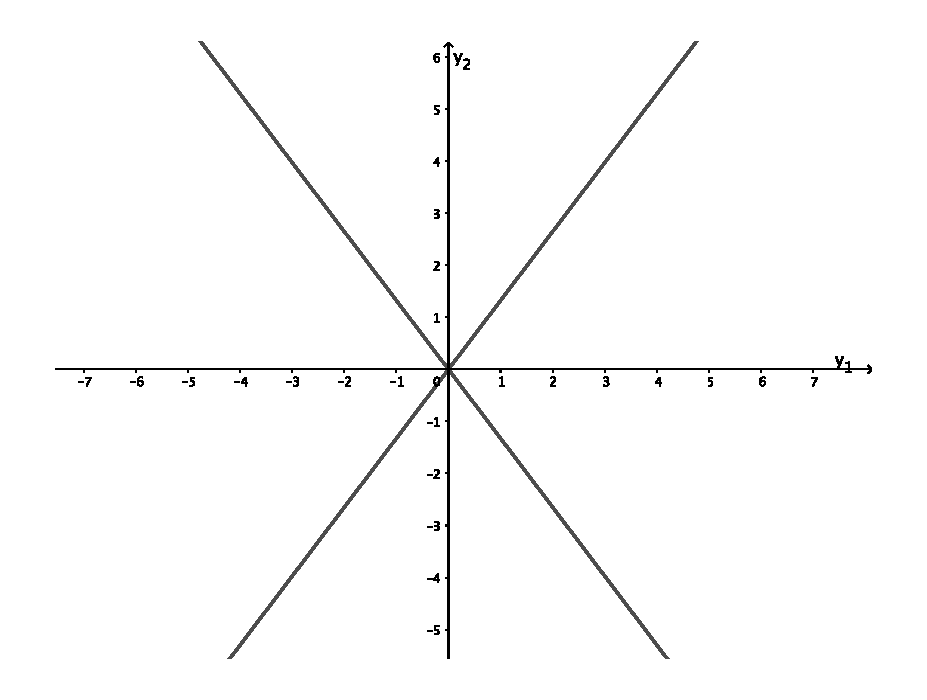
\includegraphics[width=0.5\textwidth]{a.pdf}}} 
    \subfloat[$\dfrac{y_1^2}{3} - \dfrac{y_2^2}{4} = 1$]{{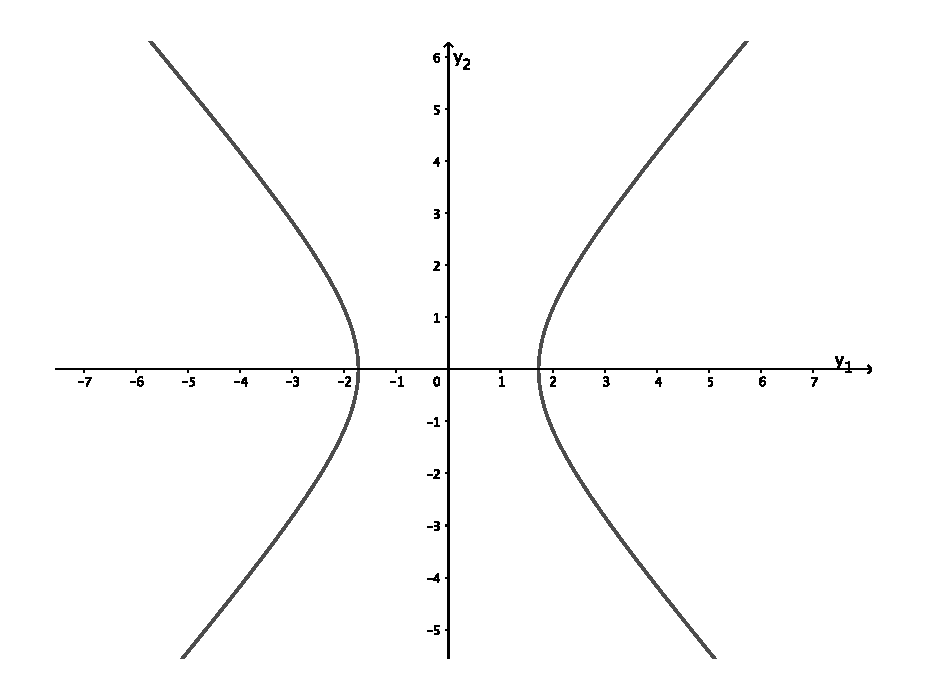
\includegraphics[width=0.5\textwidth]{b.pdf}}}
    \caption{Graphs for \textbf{Problem 4}}
\end{figure}

\section*{Problem 5}
\begin{enumerate}[leftmargin=*, label={(\alph*)}]
    \item To Prove : eigenvalues of $\mathbf{A}$ are all positive → $Q$ is positive definite
    
    $Q$ can be written in a canonical form of $\mathbf{y} = \begin{bmatrix}
        y_1 \\ \vdots \\ y_n
    \end{bmatrix}$, where $\mathbf{x} = \mathbf{Xy}$ and $\mathbf{X}$ is the orthogonal matrix with eigenvectors corresponding to eigenvalues $\qty(\lambda_1, \; \cdots, \; \lambda_n)$ as columns. 
    Since $\mathbf{x} \neq \mathbf{0}$, $\mathbf{y} \neq \mathbf{0}$ and at least one $y_i \neq 0$.

    Then $Q = \mathbf{y}^T\mathbf{Dy} = \lambda_1y_1^2 + \cdots + \lambda_ny_n^2$. 
    Since all $\lambda_i > 0$ and $\mathbf{y} \neq 0$, $Q > 0$.
    \item To Prove : $Q$ is positive definite → eigenvalues of $\mathbf{A}$ are all positive
    
    If some eigenvalue $\lambda = 0$, there is a corresponding eigenvector $\mathbf{v}$ such that $\mathbf{Ax} = \lambda\mathbf{x} = \mathbf{0}$.
    Then $\mathbf{x}^T\mathbf{Ax} = \mathbf{0}$, therefore $Q$ is not positive definite.

    If some eigenvalue $\lambda < 0$, there is a corresponding eigenvector $\mathbf{v}$ such that $\mathbf{Ax} = \lambda\mathbf{x}$.
    Then $\mathbf{x}^T\mathbf{Ax} = \mathbf{x}^T\lambda\mathbf{x} = \lambda\mathbf{x}^T\mathbf{x} = \lambda\norm{\mathbf{x}}^2 < 0$, since $\lambda < 0$ and $\mathbf{x} \neq 0$. Therefore $Q$ is not positive definite.

    Therefore, if $Q$ is positive definite, all eigenvalues of $\mathbf{A}$ are positive.
\end{enumerate}

\section*{Problem 6}
\begin{enumerate}[leftmargin=*, label={(\alph*)}]
    \item $$\frac{1}{y^2}y' = e^{2x-1}, \;\; \int\frac{1}{y^2}dy = e^{2x-1}dx$$
    $$-\frac{1}{y} = \frac{1}{2}e^{2x-1} + C', \;\; y = -\frac{2}{e^{2x-1}+C}$$
    \item $$y' = 1 + \frac{y}{x}$$
    Let $u = \dfrac{y}{x}$, then $y' = u'x + u$.
    $$u'x + u = 1 + u, \;\; u' = \frac{1}{x}$$
    $$\int1\cdot du = \int\frac{1}{x}dx$$
    $$u = \ln{x} + C$$
    $$\therefore y = x\ln{x} + Cx$$
    \item $$y' = \frac{y}{x} + 3x^3\cos^2\qty(\frac{y}{x})$$
    Let $u = \dfrac{y}{x}$, then $y' = u'x + u$.
    $$u'x + u = u + 3x^3\cos^2u, \;\; \frac{1}{\cos^2u}u' = 3x^2$$
    $$\int_0^u\frac{1}{\cos^2u}du = \int_1^x3x^2dx$$
    $$\tan{u} = x^3 - 1, \;\; u = \arctan\qty(x^3 - 1)$$
    $$\therefore y = x\arctan\qty(x^3 - 1)$$
    \item $$\qty(1 + \frac{y^2}{x^2})dx - \frac{2y}{x}dy = 0, \;\; d\qty(x - \frac{y^2}{x}) = 0$$
    $$\therefore x - \frac{y^2}{x} = C$$
    \item $$y\cos(x+y)dx + \cos(x+y)(y+\tan(x+y))dy = 0, \;\; d\qty(y\sin(x+y)) = 0$$
    $$\therefore y\sin(x+y) = C$$
    \item $$y' + \frac{4}{x}y = 8x^3, \;\; x^4y' + 4x^3y = 8x^7$$
    $$\int_{1}^{x}\qty(x^4y' + 4x^3y)dx = \int_{1}^{x}8x^7dx$$
    $$\qty[x^4y]_1^x = \qty[x^8]_1^x, \;\; x^4y - 2 = x^8 - 1$$
    $$\therefore y = x^4 + \frac{1}{x^4}$$
    \item $$\frac{y}{1-y^2}y' = x$$
    $$-\int_3^y\frac{y}{y^2-1}dy = \int_0^xxdx$$
    $$\qty[-\frac{1}{2}\ln\qty(y^2-1)]_3^y = \qty[\frac{1}{2}x^2]_0^x, \;\; \frac{1}{2}\ln\qty(\frac{8}{y^2-1}) = \frac{1}{2}x^2$$
    $$\therefore e^{x^2}\qty(y^2-1) = 8$$
\end{enumerate}

\section*{Problem 7}
We can first solve the problem in the standard way. (Nonhomogenous Linear ODE)
$$y' - y = x, \;\; e^{-x}\qty(y' - y) = e^{-x}x$$
$$\int_{0}^{x}e^{-x}\qty(y' - y)dx = \int_{0}^{x}e^{-x}xdx$$
$$\qty[e^{-x}y]_0^x = \qty[-(1+x)e^{-x}]_0^x, \;\; e^{-x}y = 1-(1+x)e^{-x}$$
$$\therefore y = e^x - x - 1$$
Now we can solve it using the Picard iteration method.
\begin{align*}
    y_n(x) &= y_0 + \int_{x_0}^{x}f\qty(t,\; y_{n-1}(t))dt \;\;\; \Big(f(x, \; y) = x + y\Big)\\
    &= \int_0^x\qty(t + y_{n-1}(t))dt
\end{align*}
We can assert $\displaystyle y_n(x) = \sum_{k=2}^{n+1}\frac{1}{k!}x^k$, and prove it using mathematical induction.
\vspace{2mm}

When $n = 0$, $y_0(x) = 0$. The statement is true.

Suppose the statement is true at $n=m \; (m \geq 0)$. Then $\displaystyle y_m(x) = \sum_{k=2}^{m+1}\frac{1}{k!}x^k$, and this gives
\begin{align*}
    y_{m+1}(x) &= \int_0^x\qty(t + y_{m}(t))dt = \int_0^x\qty(t + \sum_{k=2}^{m+1}\frac{1}{k!}t^k)dt \\
    &= \frac{1}{2}t^2 + \sum_{k=2}^{m+1}\frac{1}{(k+1)!}x^{k+1} \\
    &= \sum_{k=2}^{m+2}\frac{1}{k!}x^k
\end{align*}
Therefore the statement is true at $n = m+1$, and is true at all $n \geq 0$.
$$\therefore y = \lim_{n\to\infty}y_n(x) = \sum_{n=2}^{\infty}\frac{1}{n!}x^n = e^x - x - 1$$
We can see that the two methods give the same result for solving the ODE.

\end{document}